
\documentclass[xcolor=pdftex,dvipsnames,table,mathserif,aspectratio=169]{beamer}
\usetheme{default}
\usetheme{metropolis}
\usepackage{minted}
\usepackage{mathtools}
\setbeamersize{text margin left=.3in,text margin right=.3in} 

\DeclarePairedDelimiter\abs{\lvert}{\rvert}%
\DeclarePairedDelimiter\norm{\lVert}{\rVert}%

\usepackage[english]{babel}
\usepackage{pgf,pgfarrows,pgfnodes,pgfautomata,pgfheaps}
\usepackage{amsmath,amssymb,setspace,centernot}
\usepackage[latin1]{inputenc}
\usepackage[T1]{fontenc}
\usepackage{relsize}
\usepackage{pdfpages}
\usepackage[absolute,overlay]{textpos} 


\newenvironment{reference}[2]{% 
  \begin{textblock*}{\textwidth}(#1,#2) 
      \footnotesize\it\bgroup\color{red!50!black}}{\egroup\end{textblock*}} 

\DeclareMathSizes{10}{10}{6}{6} 

\begin{document}
\title{Part 8: Policy Evaluation- Marginal Treatment Effects}
\author{Chris Conlon}
\institute{Applied Econometrics}
\date{\today}

\maketitle
\section{Marginal Treatment Effects}

\begin{frame}{One quantity to rule them all: MTE}
\begin{itemize}
\item Consider a treatment effect $\beta_i = Y_{i}(1) - Y_{i}(0)$.
\item Think about a single-index such that $T_i = 1(v_i \leq Z_i' \gamma)$.
\item Think about the person for whom $v_i = Z_i'\gamma$ (just barely untreated).
\begin{eqnarray*}
\Delta^{MTE}(X_i, v_i) = E[\beta_i | X_i, v_i = Z_i'\gamma] 
\end{eqnarray*}
\item MTE is average impact of receiving a treatment for everyone with the same $Z' \gamma$.
\item For any single index model we can rewrite 
\begin{eqnarray*}
T_i = 1(v_i \leq Z_i' \gamma) = 1(u_{is} \leq F(Z_i' \gamma)) \mbox{ for }  u_s \in [0,1]
\end{eqnarray*}
\item $F$ is just the cdf of $v_i$
\item Now we can write $P(Z) = Pr(T=1|Z )= F(Z'\gamma)$.
\end{itemize}
\end{frame}

\begin{frame}
\frametitle{MTE: Derivation}
Now we can write,
\begin{eqnarray*}
Y_0 &=& \gamma_0' X + U_0\\
Y_1 &=& \gamma_1' X + U_1\\
\end{eqnarray*}
$P(T=1 | Z) = P(Z)$ works as our instrument with two assumptions:
\begin{enumerate}
\item $(U_0, U_1, u_s) \perp P(Z) | X$. (Exogeneity)
\item Conditional on $X$ there is enough variation in $Z$ for $P(Z)$ to take on all values $\in(0,1)$.
\begin{itemize}
\item This is much stronger than typical \alert{relevance} condition. Much more like the \alert{special regressor} method we will discus next time.
\end{itemize}
\end{enumerate}
\end{frame}

\begin{frame}
\frametitle{MTE: Derivation}
\footnotesize
Now we can write,
\begin{eqnarray*}
Y &=& \gamma_0' X + T(\gamma_1 - \gamma_0)' X + U_0 + T(U_1 - U_0)\\
E[Y| X,P(Z)=p] &=& \gamma_0' X + p(\gamma_1 - \gamma_0)'X + E[T(U_1 - U_0)|X,P(Z)=p]
\end{eqnarray*}
Observe $T=1$ over the interval $u_s = [0,p]$ and zero for higher values of $u_s$. Let $U_1-U_0 \equiv \eta$.
\begin{eqnarray*}
E[T(U_1 - U_0) | P(Z) =p,X] &=& \int_{-\infty}^{\infty} \int_{0}^{p} (U_1 - U_0) f((U_1-U_0) | U_s = u_s) d u_s d(U_1 -U_0)\\
E[T(\eta) | P(Z) =p,X] &=& \int_{-\infty}^{\infty} \int_{0}^{p} \eta f(\eta | U_s = u_s)  d\, \eta d\, u_s\\
\end{eqnarray*}
\begin{eqnarray*}
\Delta^{MTE}(p) &=& \frac{\partial E[Y | X, P(Z)=p]}{\partial p} = (\gamma_1 - \gamma_0)'X + \int_{-\infty}^{\infty} \eta f(\eta | U_s =p) d\, \eta\\
&=& (\gamma_1 - \gamma_0)'X + E[\eta | u_s =p]
\end{eqnarray*}
What is $E[\eta | u_s =p]$? The expected unobserved gain from treatment of those people who are on the treatment/no-treatment margin $P(Z)=p$.
\end{frame}

\begin{frame}
\frametitle{How to Estimate an MTE}
Easy
\begin{enumerate}
\item Estimate $P(Z) = Pr(T=1 | Z)$ nonparametrically (include exogenous part of $X$ in $Z$).
\item Nonparametric regression of $Y$ on $X$ and $P(Z)$ (polynomials?)
\item Differentiate w.r.t. $P(Z)$
\item plot it for all values of $P(Z)=p$.
\end{enumerate}
So long as $P(Z)$ covers $(0,1)$ then we can trace out the full distribution of $\Delta^{MTE}(p)$.
\end{frame}



\begin{frame}
\footnotesize
\frametitle{Everything is an MTE}
Calculate the outcome given $(X,Z)$ (actually $X$ and $P(Z)=p$).
\begin{itemize}
\item ATE : This one is obvious. We treat everyone!
\begin{eqnarray*}
\int_{-\infty}^{\infty} \Delta^{MTE}(p) = (\gamma_1 - \gamma_0)'X + \underbrace{\int_{-\infty}^{\infty} E(\eta | u_s) d\, u_s}_{0}
\end{eqnarray*}
\item LATE: Fix an $X$ and $P(Z)$ varies from $b(X)$ to $a(X)$ and we integrated over the area between (compliers).
\begin{eqnarray*}
LATE(X)=\int_{-\infty}^{\infty} \Delta^{MTE}(p) =  (\gamma_1 - \gamma_0)'X + \frac{1}{a(X)-b(X)} \int_{b(X)}^{a(X)} E(\eta | u_s) d\, u_s
\end{eqnarray*}

\item ATT 
\begin{eqnarray*}
TT(X)=\int_{-\infty}^{\infty} \Delta^{MTE}(p) \frac{Pr(P(Z | X) > p)}{E[P(Z | X)]} d\,p
\end{eqnarray*}

\item Weights for IV and OLS are a bit more complicated. See the Heckman and Vytlacil paper(s).
\end{itemize}
\end{frame}

\begin{frame}
\frametitle{Carneiro, Heckman and Vytlacil (AER 2010)}
\begin{itemize}
\item Estimate returns to college (including heterogeneity of returns).
\item NLSY 1979
\item $Y = \log(wage)$
\item Covariates $X$: Experience (years), Ability (AFQT Score), Mother's Education, Cohort Dummies, State Unemployment, MSA level average wage.
\item Instruments $Z$: College in MSA at age 14, average earnings in MSA at 17 (opportunity cost), avg unemployment rate in state.
\end{itemize}
\end{frame}


\begin{frame}
\frametitle{Carneiro, Heckman and Vytlacil}
\begin{center}
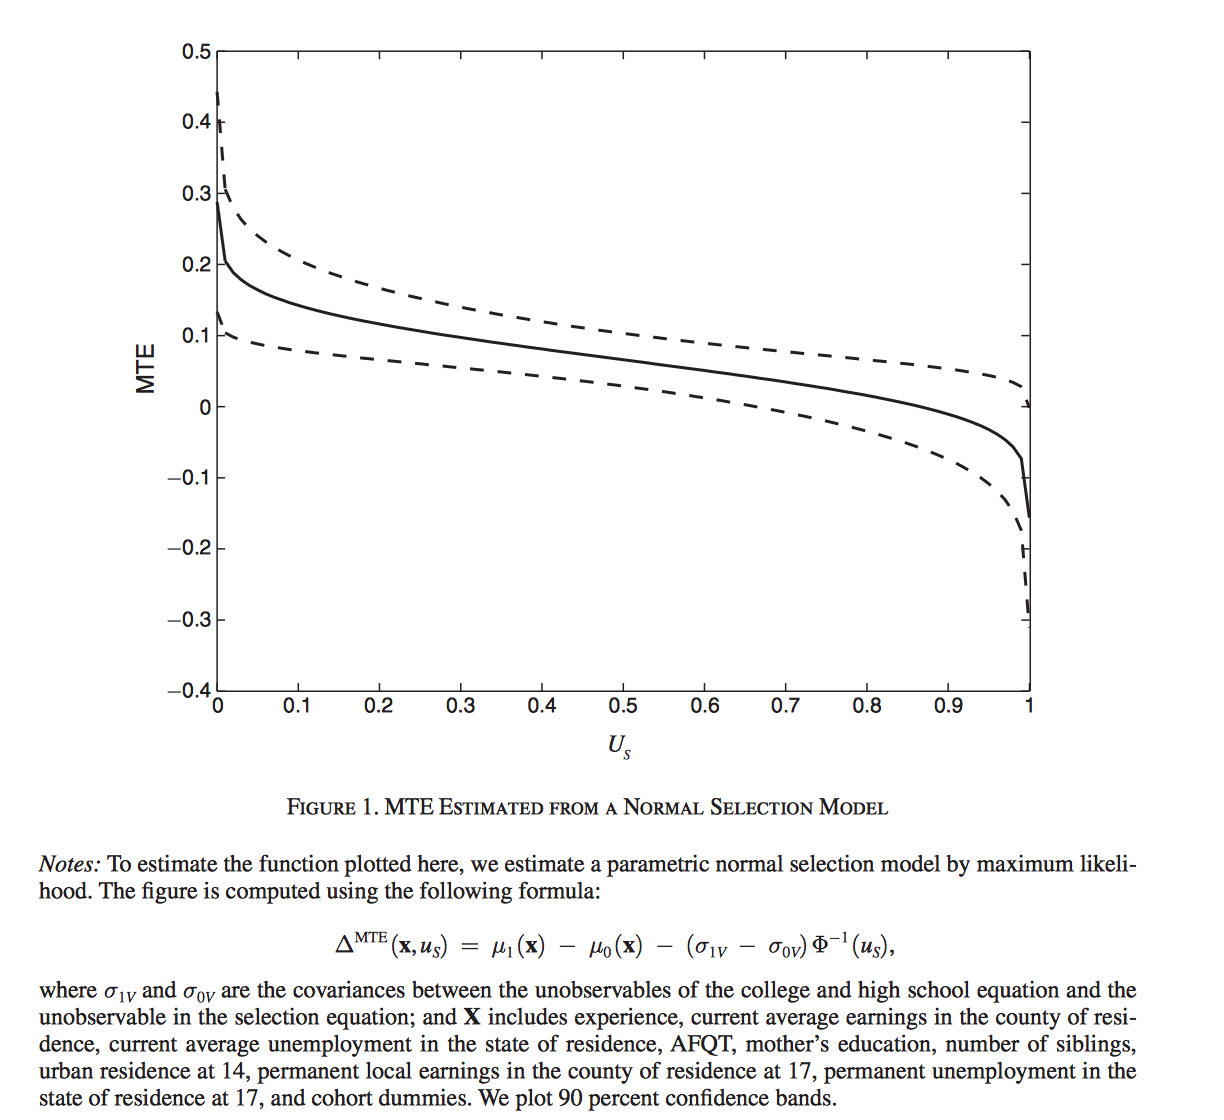
\includegraphics[width=4in]{./resources/chv_fig1}
\end{center}
\end{frame}

\begin{frame}
\frametitle{Carneiro, Heckman and Vytlacil}
\begin{center}
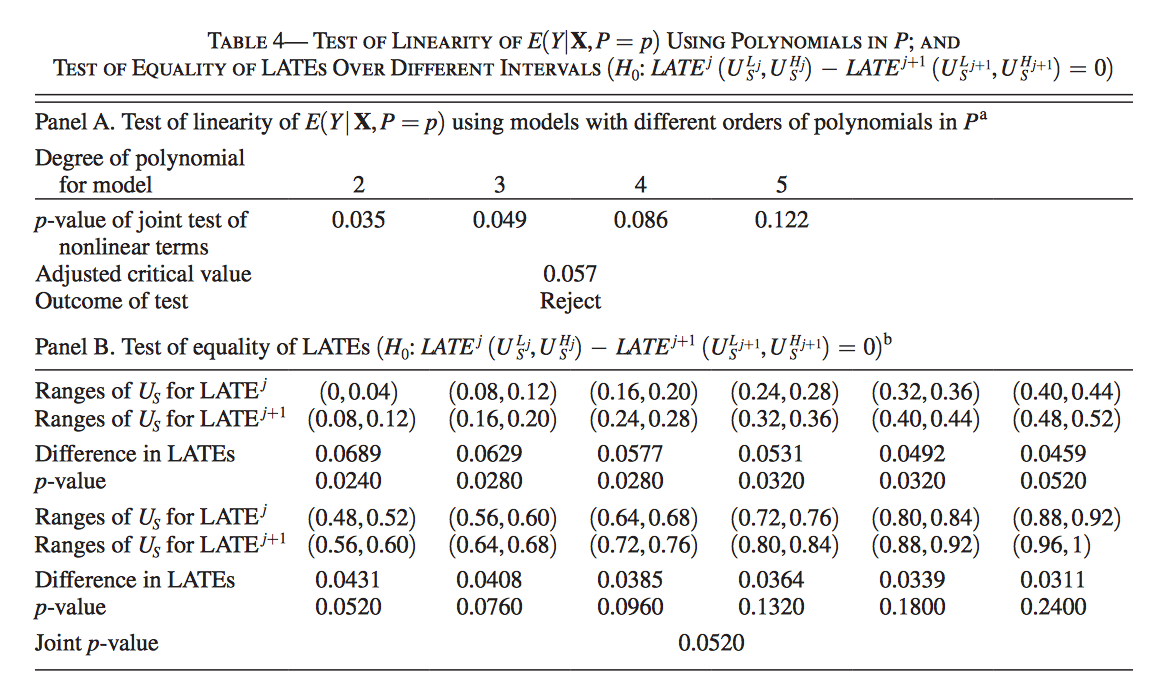
\includegraphics[width=4in]{./resources/chv_tab4}
\end{center}
\end{frame}

\begin{frame}
\frametitle{Carneiro, Heckman and Vytlacil}
\begin{center}
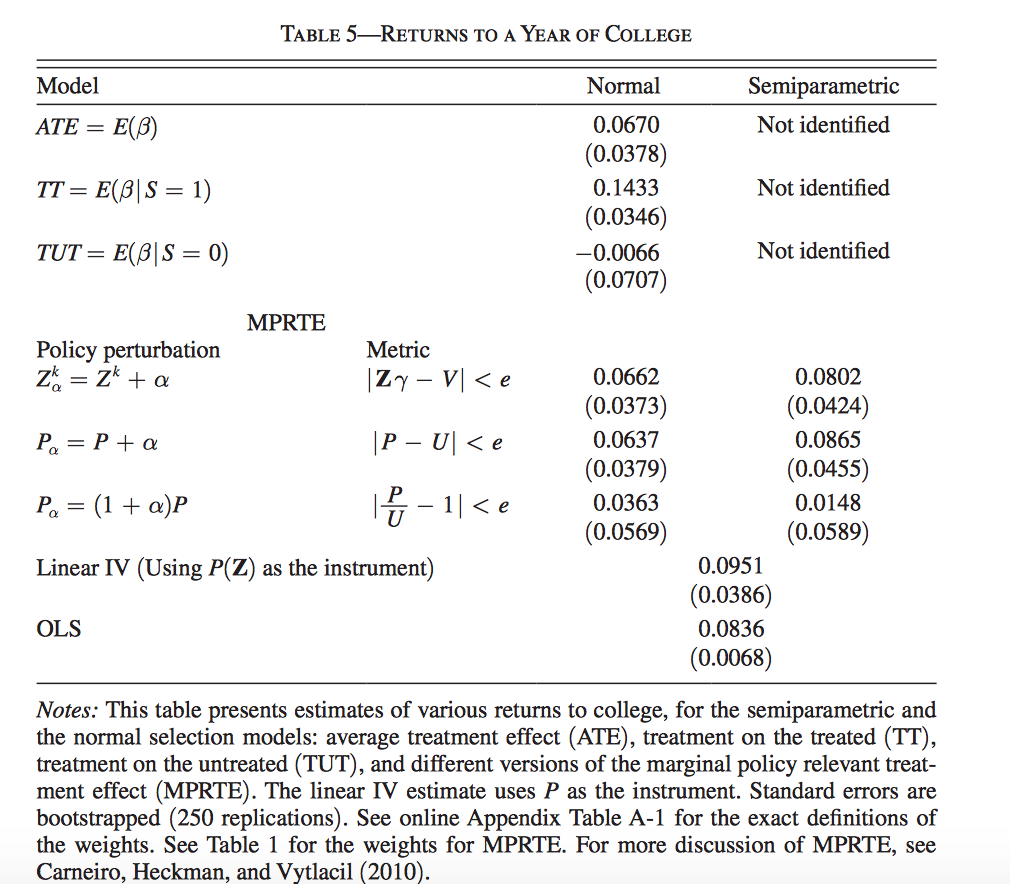
\includegraphics[width=4in]{./resources/chv_tab5}
\end{center}
\end{frame}

\begin{frame}
\frametitle{Carneiro, Heckman and Vytlacil}
\begin{center}
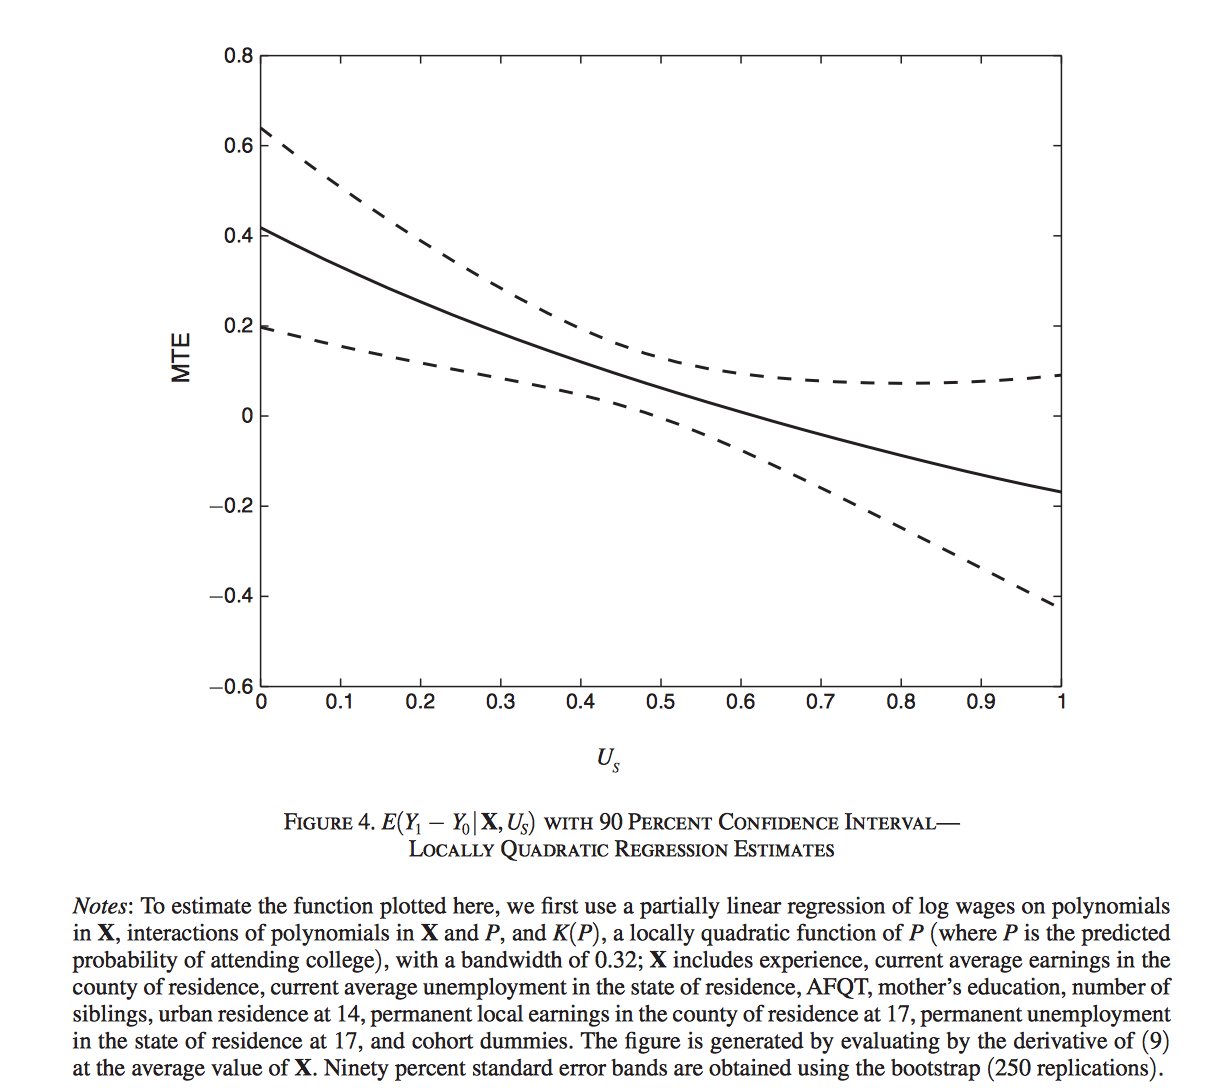
\includegraphics[width=4in]{./resources/chv_fig4}
\end{center}
\end{frame}

\begin{frame}
\frametitle{Carneiro, Heckman and Vytlacil}
\begin{center}
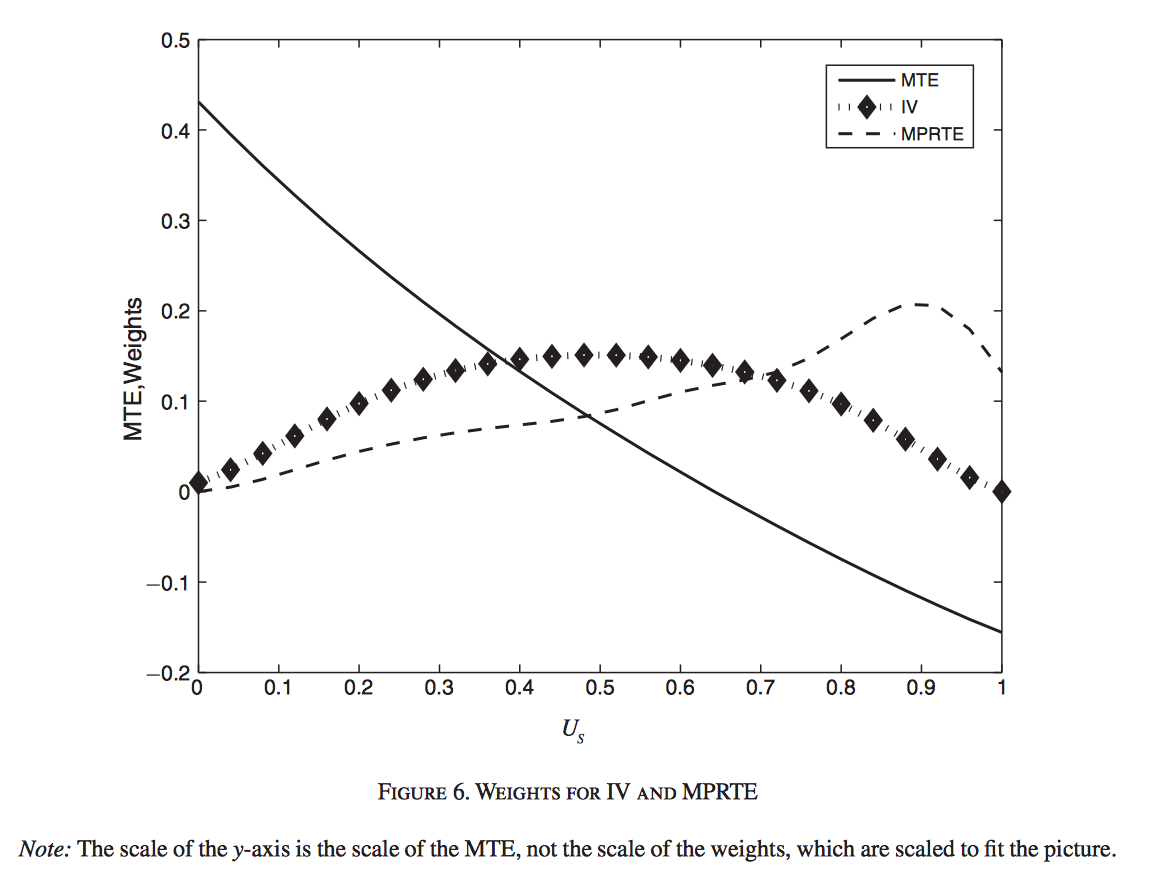
\includegraphics[width=4in]{./resources/chv_fig6}
\end{center}
\end{frame}


\begin{frame}
\frametitle{Diversion Example}
I have done some work trying to bring these methods into merger analysis.
\begin{itemize}
\item Key quantity: \alert{Diversion Ratio} as I raise my price, how much do people switch to a particular competitor's product
\begin{eqnarray*}
D_{jk}(p_j,p_{-j}) = \left| \frac{\partial q_k}{\partial p_j}(p_j,p_{-j}) /  \frac{\partial q_j}{\partial p_j}(p_j,p_{-j}) \right|
\end{eqnarray*}
\item We hold $p_{-j}$ fixed and trace out $D_{jk}(p_j)$.
\item The \alert{treatment} is leaving good $j$.
\item The $Y_i$ is increased sales of good $k$.
\item The $Z_i$ is the price of good $j$.
\item The key is that all changes in sales of $k$ come through people leaving good $j$ (no direct effects).
\end{itemize}
\end{frame}

\begin{frame}
\frametitle{Diversion for Prius (FAKE!)}
\begin{center}
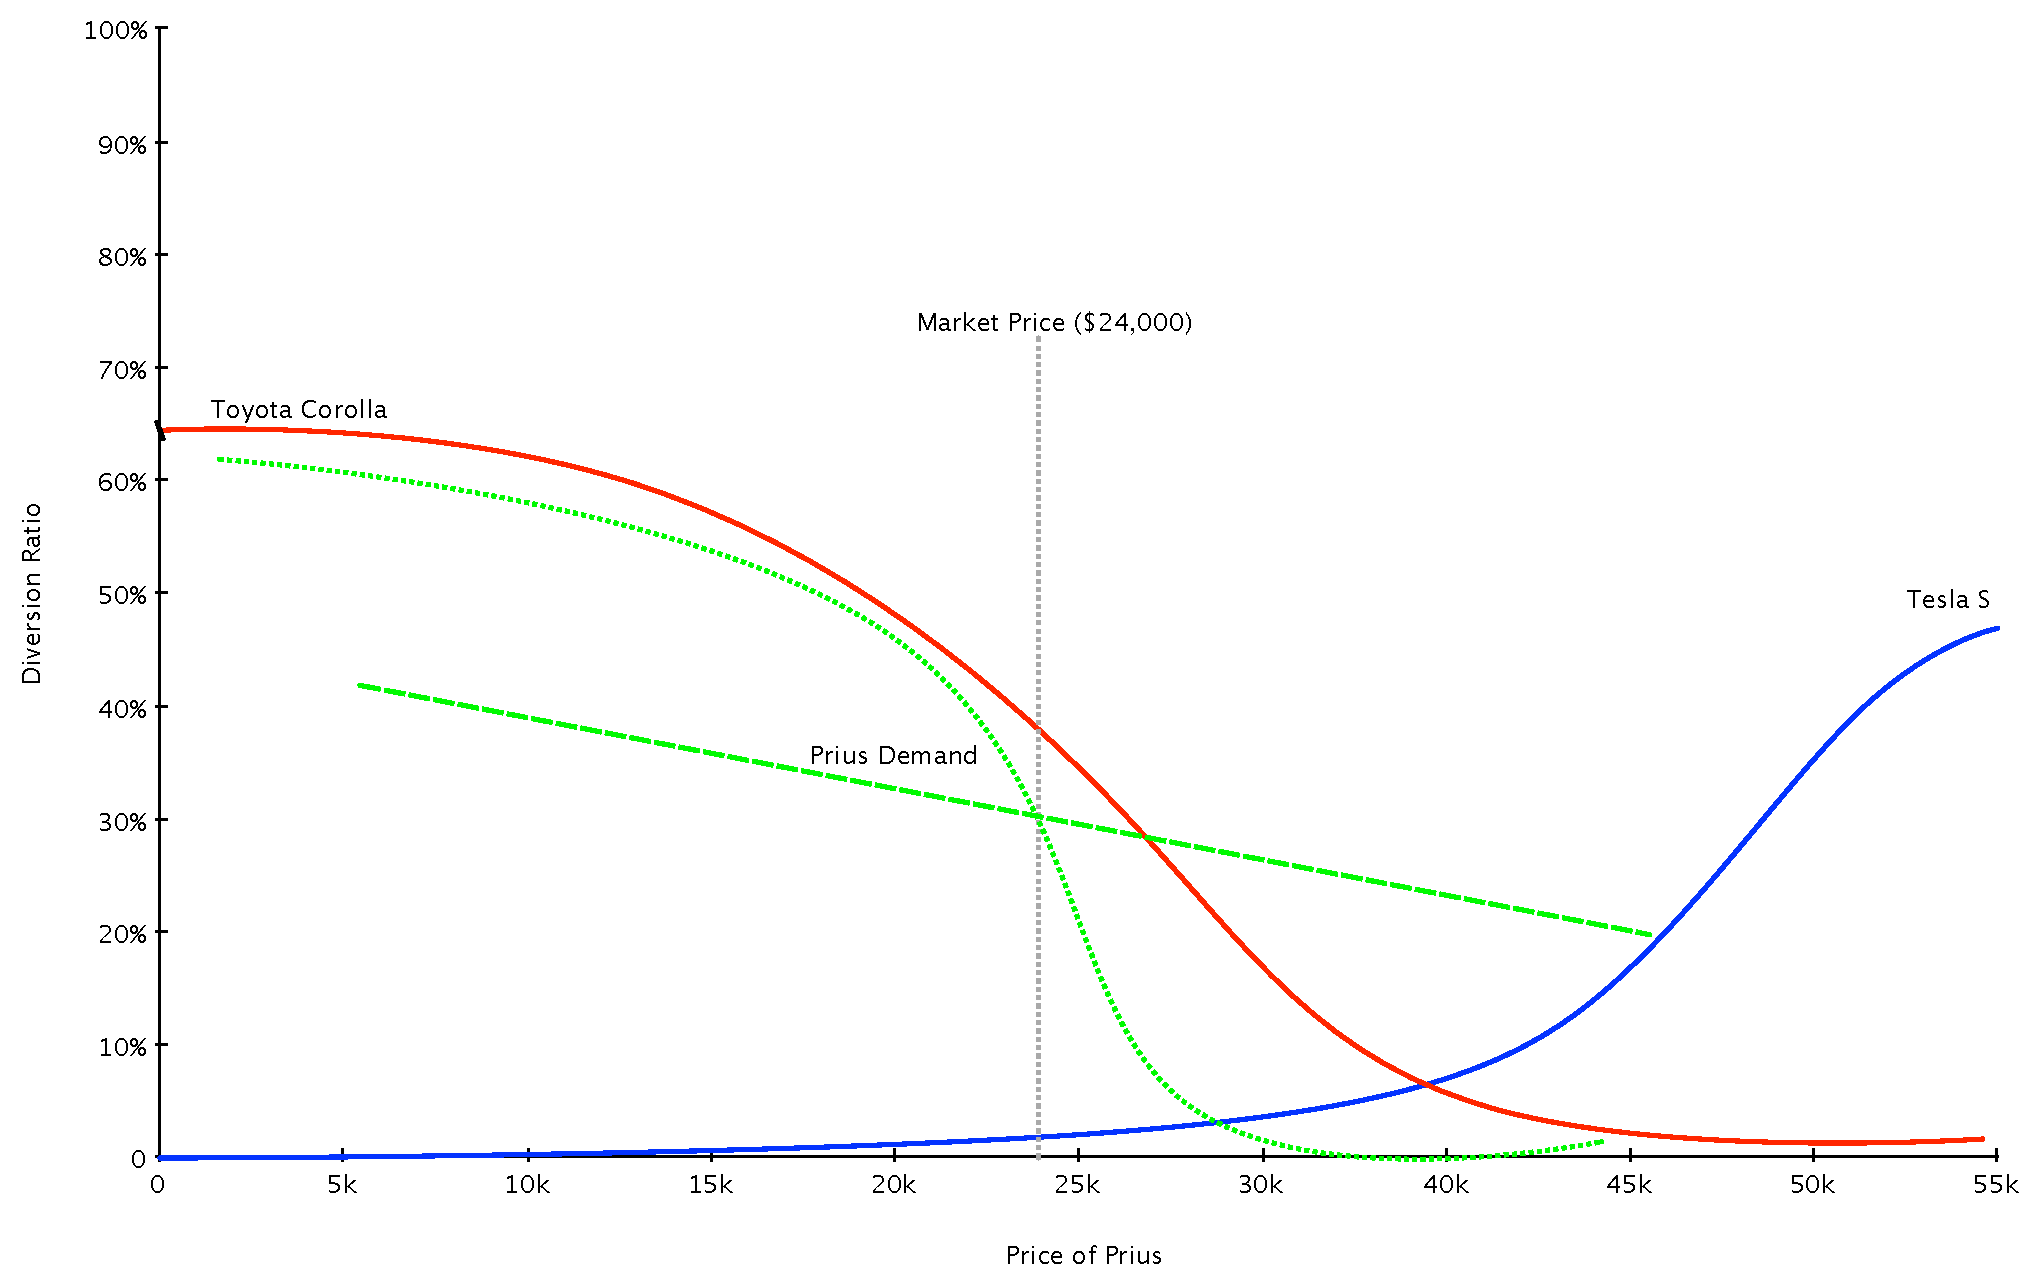
\includegraphics[width=4in]{./resources/sillydiversion.pdf}
\end{center}
\end{frame}

\begin{frame}
\frametitle{Diversion Example}
\begin{eqnarray*}
\label{weighteddiversion}
\widehat{D_{jk}^{LATE} }&=& \frac{1}{\Delta q_j} \int_{p_j^{0}}^{p_j^{0}+\Delta p_j} \underbrace{\frac{\partial q_k(p_j,p^{0}_{-j})}{\partial q_j}}_{\equiv D_{jk}(p_j,p^{0}_{-j})} \left| \frac{\partial q_j(p_j,p^{0}_{-j})}{\partial p_j} \right|\, dp_j
\end{eqnarray*}
\begin{itemize}
\item $D_{jk}(p_j,p^{0}_{-j})$ is the MTE.
\item Weights $w(p_j) = \frac{1}{\Delta q_j} \frac{\partial q_j(p_j,p^{0}_{-j})}{\partial p_j}$ correspond to the lost sales of $j$ at a particular $p_j$ as a fraction of all lost sales.
\item When is $LATE \approx ATE$? 
\begin{itemize}
\item Demand for Prius is steep: everyone leaves right away
\item $D_{j,k}(p_j)$ is relatively flat.
\item We might want to think about raising the price to choke price (or eliminating the product from the consumers choice set) same as treating everyone!
\end{itemize}
\end{itemize}
\end{frame}

\end{document}